%\documentclass[11pt,aspectratio=169]{beamer}
\documentclass[11pt]{beamer}
\usetheme{CambridgeUS}
\setbeamerfont{frametitle}{size=\small}
%\usecolortheme{dolphin}

%\setbeameroption{show notes}
%\setbeameroption{show only notes}
%\usepackage{pgfpages}
%\pgfpagesuselayout{4 on 1}[a4paper]

\usepackage[utf8]{inputenc}
\usepackage[english]{babel}
\usepackage{amsmath}
\usepackage{amsfonts}
\usepackage{amssymb}
\usepackage{graphicx}
\usepackage{subcaption}
\usepackage{algorithmic}
\captionsetup{compatibility=false}

\author{Andrew Rosen}
\title[Autonomous Load-Balancing]{Dissertation \\ Towards a Framework for DHT Distributed Computing}

\logo{
\includegraphics[height=1cm]{figs/logo}}
\institute{Georgia State University}
\date{May 13th, 2016}
%\subject{}
%\setbeamercovered{transparent}
%\setbeamertemplate{navigation symbols}{}



\AtBeginSection[]
{
  \begin{frame}
    \frametitle{Table of Contents}
    \tiny{\tableofcontents[currentsection]}
  \end{frame}
}

\begin{document}
	
	
	
\maketitle


\section{Introduction}


\subsection{Objective}
\begin{frame}{Objective}

\begin{itemize}
	\item Our objective is to create a generalized framework for distributed computing using Distributed Hash Tables.
\end{itemize}
\pause
\begin{center}
	Or
\end{center}

\pause
We want to build a completely decentralized distributed computing framework.
\end{frame}

\note[itemize]{
	\item We want to build a completely decentralized distributed computing framework based on distributed hash tables, or DHTs.
	\item Doing this will require a generic framework for creating distributed hash tables and distributed applications.
	\item This means we need two things:
	\item A way of easily abstracting DHTs 
	\item A way to make sure that we can distribute work effectively across a DHT
}

\subsection{Distributed Computing and Challenges}

\begin{frame}{What do I Mean by Distributed Computing?}
	A system where we can take a task and break it down into multiple parts, where each part is worked upon individually.
\end{frame}

\note{A distributed computing framework is a system where we can take a job, break in up into smaller pieces, and send these pieces out to be worked upon by computing agents.}

\begin{frame}{Challenges of Distributed Computing}
	Distributed Computing platforms experience these challenges:
	\begin{description}
		\item<1->[Scalability] As the network grows, more resources are spent on maintaining and organizing the network. 
		\note<1>{Remember, computers aren't telepathic. There's always an overhead cost.  It will grow.   The challenge of scalability is designing a protocol  in which this cost grows at an extremely slow rate. 
			For example, a single node keeping track of all members of the system might be a tenable situation up to a certain point, but eventually, the cost becomes too high for a single node.}
		\item<2->[Fault-Tolerance] As more machines join the network, there is an increased risk of failure. \note<2>{Failure Hardware failure is a thing that can happen. Individually the chances are low, but this becomes high when we're talking about millions of machines.  Also, what happens in a P2P environment.  Nodes leaving is treated as a failure.}  
		\item<3->[Load-Balancing] Tasks need to be evenly distributed among all the workers. \note<3>{If we are splitting the task into multiple parts, we need some mechanism to ensure that each worker gets an even (or close enough) amount of work.}
	\end{description}
	
\end{frame}


\subsection{What Are Distributed Hash Tables?}

\begin{frame}{Distributed Key/Value Stores}
	\textbf{Distributed Hash Tables }are mechanisms for storing values associated with certain keys.
	\begin{itemize}
		\item Values, such as filenames, data, or IP/port combinations are associated with keys.
		\item These keys are generated by taking the hash of the value.
		\item We can get the value for a certain key by asking any node in the network.
	\end{itemize}
\end{frame}

\note{At their core, Distributed Hash Tables are giant lookup  tables.  Given a key, it will return the value associated with that key, if it exists.
These keys, or hash keys, are generated by a hash function, such as SHA1 or MD5.
These hash functions use black magic using prime numbers and modular arithmetic to return a close to unique identifier associated with a given input.
The key about the keys is the same input will always produce the same output.
From a probability standpoint, they are distributed uniformly at random.
}



%\begin{frame}{How Does It Work?}
%	
%	\begin{itemize}
%		\item DHTs organize a set of nodes, each identified by an \textbf{ID}. 
%		\item Nodes are responsible for the keys that are closest to their IDs.
%		\item Nodes maintain a small list of other peers in the network.
%		\begin{itemize}
%			\item Typically a size $ \log(n)$ subset of all nodes in the network.
%		\end{itemize}
%		\item Each node uses a very simple routing algorithm to find a node responsible for any given key.  %Explain what that is
%	\end{itemize}
%\end{frame}
%
%\note[itemize]{
%
%\item We'll explain in greater detail later, but briefly:
%\item DHTs are composed of a set of nodes, each identified by a hashed ID
%\item Each node is responsible for the key/value pairs that fall within its zone of responsibility, which can be thought of as the nodes closest to it/.
%\item Nodes keep a list of other nodes in the network, composed of peers that are close to it in terms of ID, and shortcuts to achieve sublinear lookup time.
%\item To lookup a particular key, the node asks ``Am I responsible for this key?'' If yes, yay! If no, I forward this message to the peer I know who I think is best able answer this question.
%}
%
%
%\begin{frame}{Current Applications}
%	Applications that use or incorporate DHTs:
%	\begin{itemize}
%		\item P2P File Sharing applications, such as BitTorrent.
%		\item Distributed File Storage.
%		\item Distributed Machine Learning.
%		\item Name resolution in a large distributed database.
%	\end{itemize}
%\end{frame}
%
%\note[itemize]{
%	\item DHTs weren't necessarily designed with large-scale P2P applications in mind, but that use case was never ignored.
%	\item BitTorrent uses a DHT, called MainlineDHT, and has about 20 million nodes active at any given time, and has a churn of about 50 \% per day.
%
%}

%\begin{frame}{Strengths of DHTs }
%	DHTs are designed for large P2P applications, which means they need to be (and are):
%	\begin{itemize}
%		\item[Scalable] 
%		\begin{itemize}
%			\item Each node knows a \emph{small} subset of the entire network.
%			\item Join/leave operations impact very few nodes.
%		\end{itemize}
%		\item[Fault-Tolerant] 
%		\begin{itemize}
%			\item The network is decentralized.
%			\item DHTs are designed to handle \alert{churn}.
%
%		\end{itemize}
%		\item[Load-Balancing]
%		\begin{itemize}
%			\item Consistent hashing ensures that nodes and data are close to evenly distributed.
%			\item Nodes are responsible for the data closest to it.
%		\end{itemize}
%	\end{itemize}
%	
%\end{frame}
\subsection{Why DHTs and Distributed Computing}

\begin{frame}{Strengths of DHTs }
	DHTs are designed for large P2P applications, which means they need to be (and are):
	\begin{itemize}
		\item Scalable
		\item Fault-Tolerant
		\item Load-Balancing
	\end{itemize}
	
\end{frame}

\note[itemize]{
	\item Scalability 
	\begin{itemize}
		\item Each node knows a \emph{small} subset of the entire network.
		\item Join/leave operations impact very few nodes.
		\item The subset each node knows is such that we have expected $ \lg(n) $ lookup
	\end{itemize}

}

\note[itemize]{
		\item Fault-Tolerance 
		\begin{itemize}
			\item The network is decentralized.
			\item DHTs are designed to handle churn.
			\item Because Joins and node failures affect only nodes in the immediate vicinity, very few nodes are impacted by an individual operation.
		\end{itemize}
		\item Load Balancing
		\begin{itemize}
			\item Consistent hashing ensures that nodes and data are close to evenly distributed.
			\item This allows a large-scale failure, like California being hit by a massive earthquake, to be absorbed throughout the network, rather than a contiguous portion being knocked out.
			\item Nodes are responsible for the data closest to it.
			\item The space is large enough to avoid Hash collisions.
		\end{itemize}	 
}



\section{Background}

\subsection{The Components and Terminology}


\begin{frame}{Required Attributes of DHT}
	\begin{itemize}
		\item A distance function.
		\item A closeness or ownership definition.
		\item A Peer management strategy.
	\end{itemize}
\end{frame}

\note[itemize]{
	\item There needs to be a way to establish how far things are from one another.
	Once we have a distance metric, we define what we mean when we say a node is responsible for all data \textit{close} to it.
	\item The closeness metric establishes how a node decides what it is responsible for.
	\item The peer management strategy encompasses a whole lot: the network topology, the distribution of long links (are they organized and spread out over specified  intervals, are they chosen according to a random distribution?), and the network maintenance.
	}

\begin{frame}{Terms and Variables}
	\begin{itemize}
		\item Network size is $n$ nodes.
		\item Keys and IDs are $m$ bit hashes, usually SHA1.
		\item Peerlists are made up of:
		\begin{description}
			\item[Short Peers] The neighboring nodes that define the network's topology.
			\item[Long Peers] Routing shortcuts.
		\end{description}
	\end{itemize}
\end{frame}

\note[itemize]{
	\item SHA1 is being depreciated, but this is trivial from our perspective.  
	\item Short peers are actively maintained, long peers replaced gradually and are not actively pinged.
}





\subsection{Example DHT: Chord}

\begin{frame}{Chord}
	\begin{itemize}
		\item Ring Topology
		\item Short Peers: predecessor and successor in the ring.
		\item Responsible for keys between their predecessor and themselves.
		\item Long Peers:  $\log n$ nodes, where the node at index $i$ in the  peerlist is 
		$$ root(r + 2^{i-1} \mod  m) ,  1 < i  < m $$
		
		
		
	\end{itemize}
\end{frame}

\note[itemize]{
	\item Chord is a favorite because we can draw it.
	\item Draw a Chord network on the wall?
	\item node $r$ is our root node.
	\item $ i $ is the index on the list
	\item English for the equation, the long peers double in distance from the root node, allowing us to cover at least half the distance to our target in a step
	\item In this way, we can achieve an expected $ \lg n $  hops. 
}

\begin{frame}{A Chord Network}
	\begin{figure}
		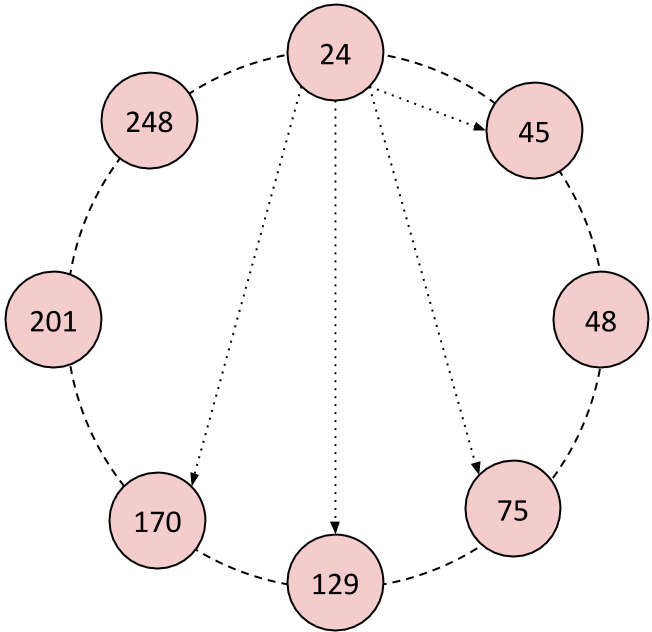
\includegraphics[width=0.55\linewidth]{figs/CR_overlay}
		\caption{An 8-node Chord ring where $m=8$.  Node 24's long peers are shown.}
		\label{fig:chordreal}
	\end{figure}
\end{frame}

\note[itemize]{
	\item The dashed lines are the short links; each node keeps track of its successor and predecessor.
	\item The dotted lines are node 24's long links; since $ m = 8$  there's 8, but since the network is so small,  4 are duplicates.
	\item Traffic travels clockwise.
	\item Routing example 24 to 150.
	}
%
%\begin{frame}{Fault Tolerence in Chord}
%	\begin{itemize}
%		\item Local maintenance thread  gradually fixes the network topology.
%		\begin{itemize}
%			\item Each node ``notifies'' its successor.
%			\item The successor replies with a better successor if one exists.
%		\end{itemize}
%		\item The long peers are gradually updated by performing a lookup on each entry.
%		
%	\end{itemize}
%\end{frame}
%
%\note[itemize]{
%	\item The notification allows a sucessor to either update its predecessor if incorrect and the predecessor to update its successor if wrong
%	\item Some implementations use predecessor and successor lists.
%	\item The long peers are replaced much slower; maintenance slowly iterates through the long peers and queries to see if there's better node for that particular long peer.
%}
%
%\begin{frame}{Handling Churn in General}
%	\begin{itemize}
%		\item Short peers, the neighbors, are regularly queried to:
%		\begin{itemize}
%			\item See of the node is still alive.
%			\item See if the neighbor knows about better nodes.
%		\end{itemize}
%		\item Long peer failures are replaced by periodic maintenance.
%	\end{itemize}
%\end{frame}
%
%
%\note[itemize]{
%	\item Short peers need to be actively maintained to keep the topology correct.
%	\item Long peers can either be replaced when a failure is detected, or periodically updated at a slower rate than the short peers.
%}
%\subsection{Other DHTs}
%\begin{frame}{Other DHTs}
%	Other DHTs include
%	\begin{itemize}
%		\item Kademlia 
%		\item Pastry and Tapestry
%		\item CAN
%		\item Symphony %
%		\item ZHT
%	\end{itemize}
%\end{frame}


\section{Completed Work}
%TODO Make one to two slides per chapter of previous work

\begin{frame}{Overarching Theme}
My research has been focused on:
	\begin{itemize}
		\item Abstracting out DHTs.
		\item Distributed computation using DHTs.
	\end{itemize}
\end{frame}

\note[itemize]{
	\item I want to get down to what the essence of a DHT is, find out what all DHTs have in common, so that I could create a generic DHT.
	\item As I implied earlier, we all these DHTs, but they all have the same features, and I want to generalize them.
	\item I focused on creating a more abstract framework for MapReduce, so I could move it out of the datacenter and into other contexts.
}

\begin{frame}{ChordReduce}
Objective:
\begin{itemize}
	\item Create an abstract MapReduce framework.
	\item Create a completely decentralized, fault-tolerant, distributed computing framework. 

\end{itemize}

Results:
\begin{itemize}
	\item We succeeded.
	\item Our network could handle nodes leaving, as well as assign joining nodes work.
	\item We found anomalous results with Churn.
\end{itemize}

\note[itemize]{
\item We leveraged Chord's fault tolerance mechanisms to handle tasks 
\item Why did churn do what it did?  That's covered in Autonomous Load Balancing.
}

\end{frame}

\begin{frame}{VHash and DGVH}



What was it:
\begin{itemize}
	\item Made a Voronoi-based DHT.
	\item A greedy heuristic.
	\item More detail later.
\end{itemize}


Results:
\begin{itemize}
	\item New concept: nodes that move their position.
	\item DGVH.
	\item We started to think how about how can we completely abstract any DHT topology into a Voronoi/Delaunay relationship.
\end{itemize}

\end{frame}


\begin{frame}{D$^3$NS}

\begin{itemize}
	\item Create a completely decentralized, distributed, DNS.
	\item Backwards compatible and completely reliable to the user.
	\item Used Blockchains and UrDHT.
\end{itemize}
\end{frame}


\begin{frame}{Sybil Attack Analysis}
\begin{itemize}
	\item Studied the amount of resources needed to perform a Sybil attack.
	\item Examined how difficult it was for nodes to inject a Sybil into a specific location.
\end{itemize}


\end{frame}



\section{UrDHT}

\subsection{Introduction}
\begin{frame}{Introduction}
	\begin{itemize}
		\item Build on DGVH and VHash
		\item Create an abstract model of a DHT based on Voronoi/Delaunay 
		\item Can be used as a bootstrapping network for other distributed systems
		\item Can emulate the topology of other DHTs
	\end{itemize}
\end{frame}





\subsection{DGVH}


\begin{frame}{Goals}
	VHash and DGVH sprung from two related ideas:
	\begin{itemize}
		
		\item<1-> We wanted a way be able optimize latency by embedding it into the routing overlay. \note<1>{Most DHTs optimize routing for the number of hops, rather than latency.}
		\item<2-> We wanted to create a DHT based off of Voronoi tessellations. Unfortunately: \note<2>{ We discovered a mapping between Distributed Hash Tables and Voronoi/Delaunay Triangulations.}
		\begin{itemize}
			\item<3-> Distributed algorithms for this problem don't really exist.  \note<3>{I lie, they do exist, but they all are ``run the global algorithm on your local subset.  And if we move out of or above 2D Euclidean space, as Brendan wanted to, no fast algorithms exist at all.  We quickly determined that solving was never really a feasible option. So that leaves approximation.  A distributed algorithm would be helpful for some WSNs solving the boundary coverage problem.}
			\item<4-> Existing approximation algorithms were unsuitable. \note<4>{Simple approximations have no guarantees of connectivity, which is very bad for a routing topology.  Better algorithms that existed for this problem technically ran in constant time, but had a prohibitively high sampling.  So to understand what I'm talking about here, let's briefly define what a Voronoi tessellation is.}
		\end{itemize}
		%		\item<5>  We wanted to the nodes to move in the key space to adjust to . \note{Just a minor challenge no }
	\end{itemize}
\end{frame}


\begin{frame}{Voronoi Tesselation}
	\begin{figure}
		\centering
		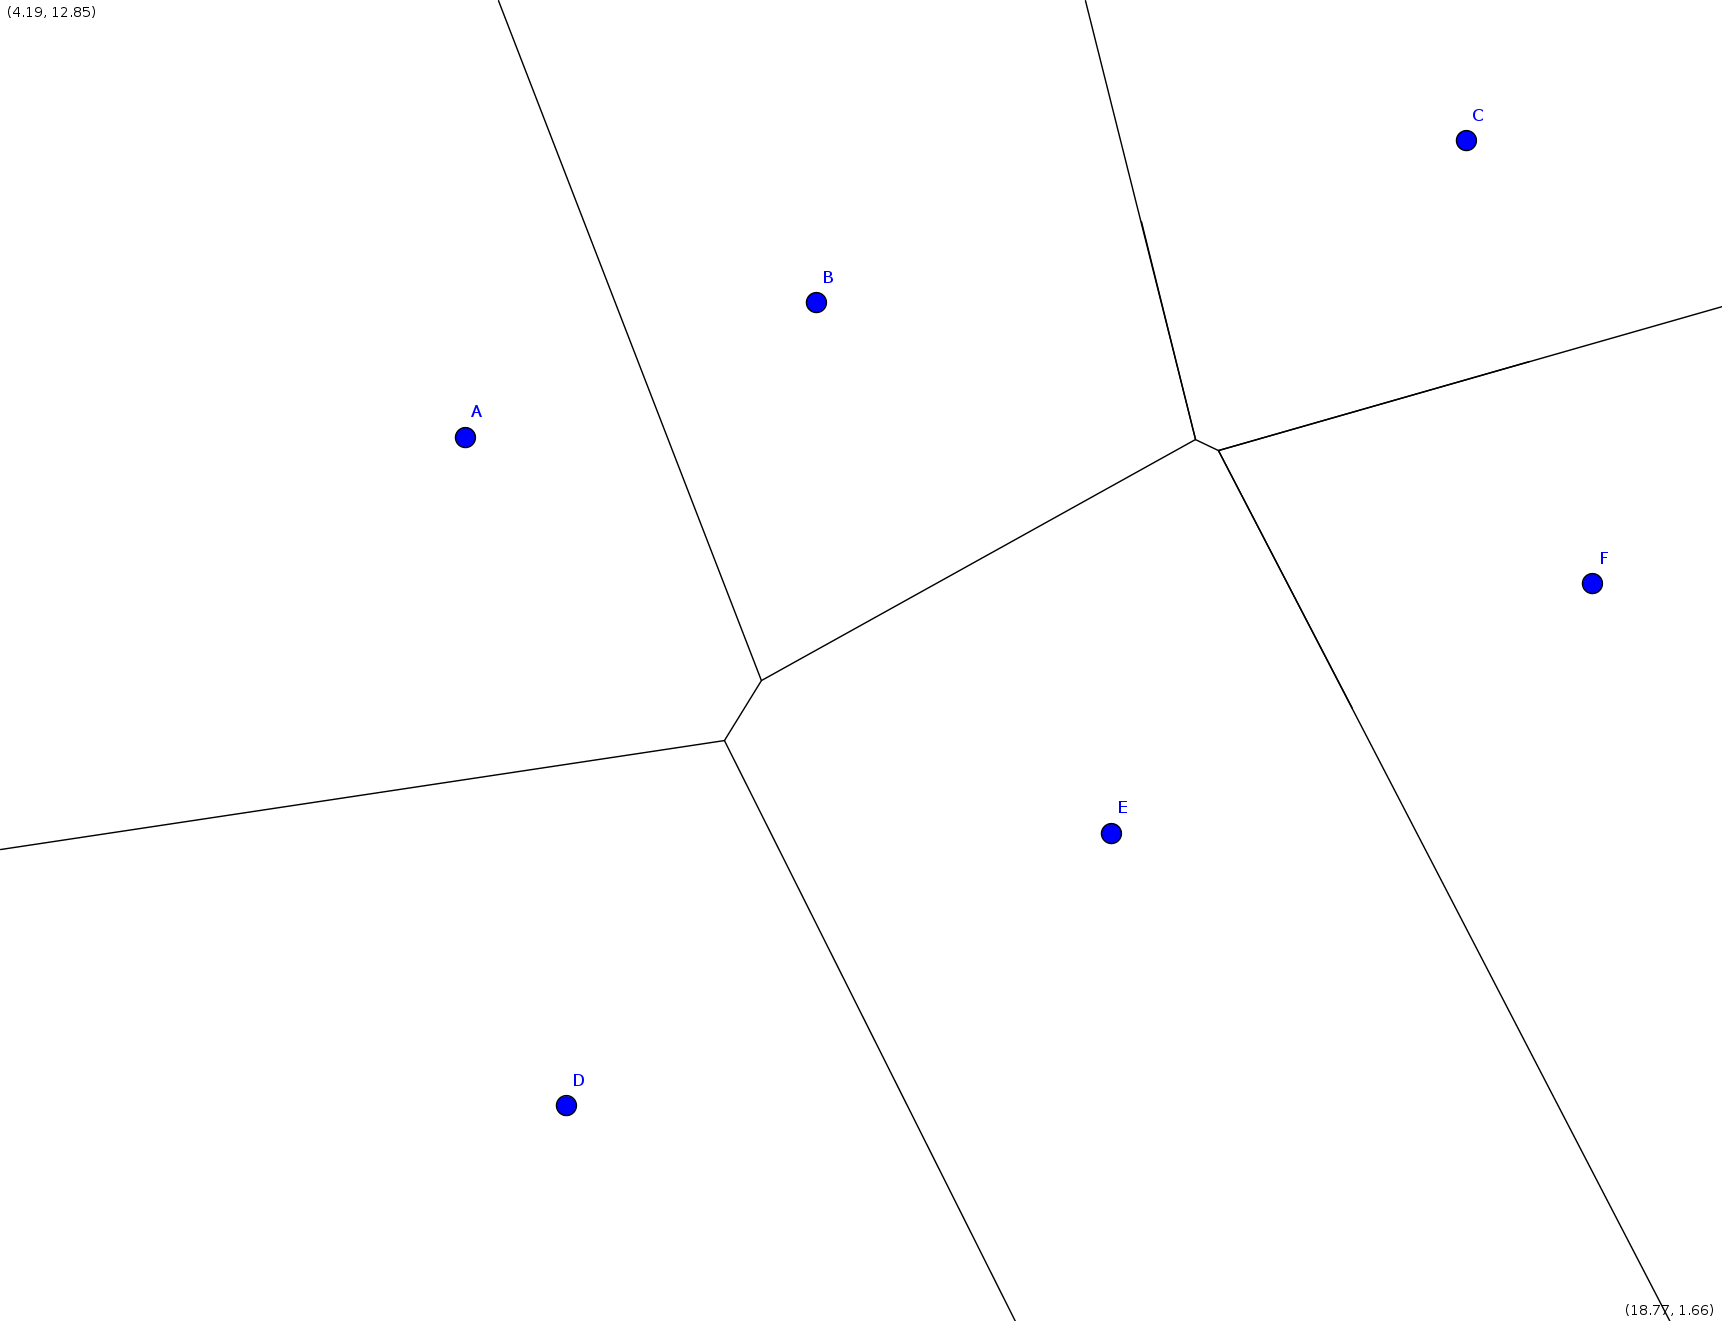
\includegraphics[width=0.9\linewidth]{figs/new_voronoi}
		%\caption{A set of points and the generated Voronoi regions}
		\label{fig:new_voronoi}
	\end{figure}
\end{frame}

\note{Define
	\begin{itemize}
		\item A Voronoi tessellation or Voronoi diagram divides a space into regions, where each region encompasses all the points closest to Voronoi generators (point).
		\item Voronoi generators
		\item Voronoi Region
		\item Voronoi Tessellation/ Diagram
	\end{itemize}
}

\begin{frame}{Delaunay Triangulation}
	\begin{figure}
		\centering
		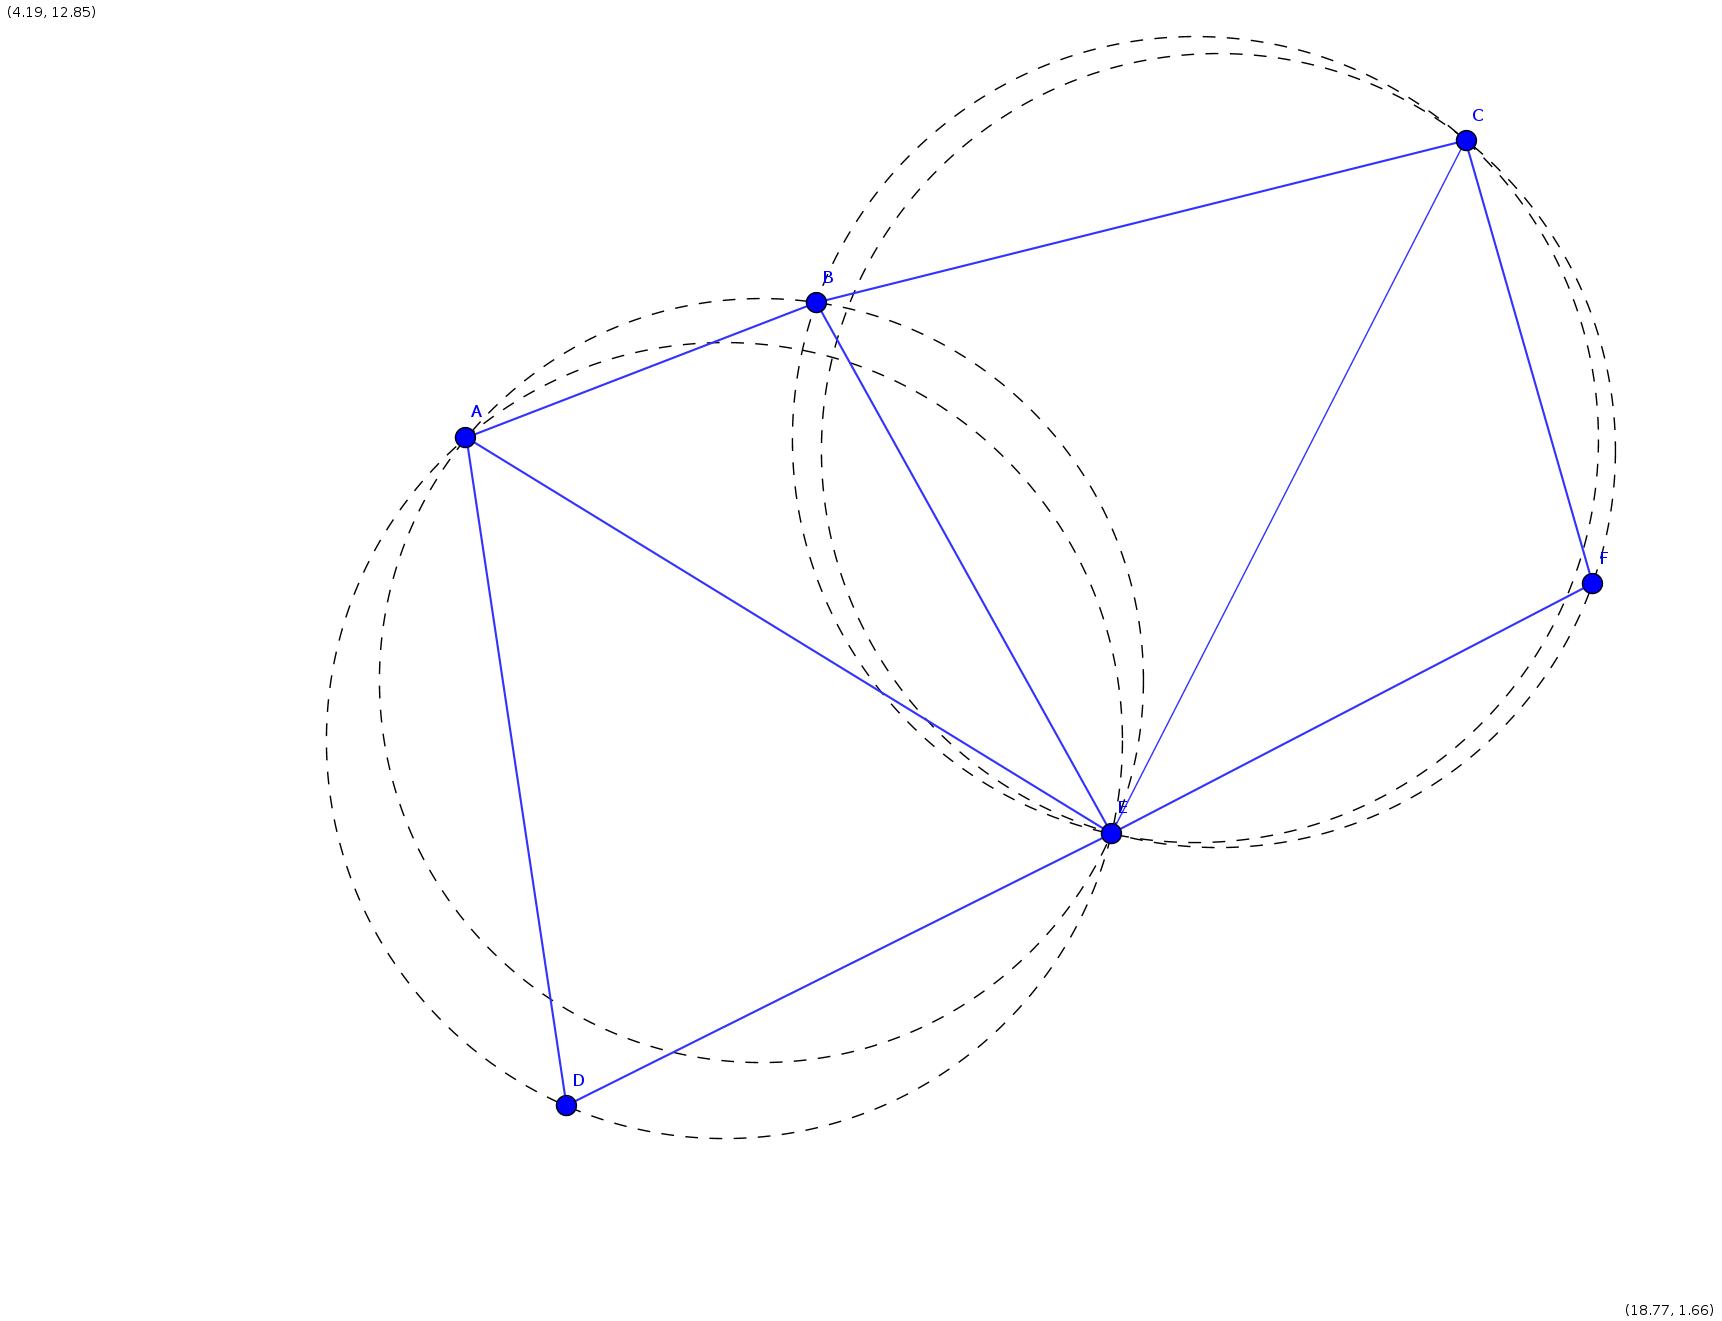
\includegraphics[width=0.9\linewidth]{figs/delaunay}
		%\caption{The same set of nodes with their corresponding Delaunay Triangulation.}
		\label{fig:delaunay}
	\end{figure}
\end{frame}

\note{Define
	\begin{itemize}
		\item Delaunay Triangulation is a triangulation of a set of points with the following rule:
		\item No point falls within any of the circumcircles for every triangle in the triangulation, 
		\item The Voronoi tessellation and Delaunay Triangulation are dual problems.
		\begin{itemize}
			\item Solving one yields the other.
			\item We can get the Voronoi diagram by connecting all the centers of circumcircles.
		\end{itemize}
	\end{itemize}
}


\begin{frame}{DHT and Voronoi Relationship }
	\begin{itemize}
		\item We can view DHTs in terms of Voronoi tessellation and Delaunay triangulation.
		\begin{itemize}
			\item The set of keys the node is responsible for is its Voronoi region.
			\item The nodes neighbors are its Delaunay neighbors.
		\end{itemize}
	\end{itemize}
\end{frame}

\note{
	It turns out we  can look at distributed hash tables in terms of Voronoi tessellation and Delaunay triangulation. 
	So if we have a quick way approximate this, we can build a DHT based directly on Voronoi tessellation and Delaunay triangulation.
}


\begin{frame}{Distributed Greedy Voronoi Heuristic}
	
	\begin{itemize}
		\item Assumption: The majority of Delaunay links cross the corresponding Voronoi edges.
		\item We can test if the midpoint between two potentially connecting nodes is on the edge of the Voronoi region.
		\item This intuition fails if the midpoint between two nodes does not fall on their Voronoi edge.
	\end{itemize}
	
\end{frame}

\begin{frame}{DGVH Heuristic}
	
	\begin{algorithmic}[1]  % the numberis how many lines
		\STATE Given node $n$ and its list of $candidates$.
		\STATE $peers \leftarrow$ empty set that will contain $n$'s one-hop peers
		\STATE Sort $candidates$ in ascending order by each node's distance to $n$
		\STATE Remove the first member of $candidates$ and add it to $peers$
		\FORALL{$c$ in $candidates$}
		\IF{Any node in $peers$ is closer to $c$ than $n$}
		\STATE Reject $c$ as a peer
		\ELSE
		\STATE Remove $c$ from $candidates$
		\STATE Add $c$ to $peers$
		\ENDIF
		\ENDFOR
	\end{algorithmic}
	
\end{frame}



\note{
	\begin{enumerate}
		\item We have $ n$, the current node and a list of candidates.
		\item  peers is a set that will build the peerlist in
		\item We sort the candidates from closest to farthest.
		\item The closest candidate is always guaranteed to be a peer.
		\item Next, we iterate through the sorted list of candidates and either add them to the peers set or discard them.
		\item If the  candidate is closer to any peer than $n$, then it does not fall on the interface between the location's Voronoi regions.
		\item in this case discard it
		\item otherwise add it the current peerlist
	\end{enumerate}
}


\begin{frame}{DGVH Time Complexity}
	For $ k $ candidates, the cost is: 
	\[ k\cdot\lg(k)  + k^{2} \text{ distances} \]
	
	However, the expected maximum for $k$ is $\Theta(\frac{\log n}{\log \log n} )$, which gives an expected maximum cost of 
	
	\[ O(\frac{\log^{2} n}{\log^{2} \log n} ) \]
	or
	\[O(\frac{\log^{4} n}{\log^{4} \log n} )\]
	
	Depending on whether we gossip with a single neighbor or all neighbors.
	
\end{frame}

\note{
	DVGH is very efficient in terms of both space and time.
	Suppose a node $n$ is creating its short peer list from $k$ candidates in an overlay network of $N$ nodes.
	The candidates must be sorted, which takes $O(k\cdot\lg(k))$ operations.
	Node $n$ then compares distances between all peers  and all the candidates.
	This results in a cost of
	
	\[ k\cdot\lg(k) + k^{2} \text{ distances} \]
	
	
	Since $k$ is  bounded by $\Theta(\frac{\log N}{\log \log N} )$ (the expected maximum degree of a node), we can translate the above to:
	
	
	The expected worst case cost of DGVH is \(O(\frac{\log^{4} n}{\log^{4} \log n} )\), if we swap with all short peers.
	Otherwise the cost is $O(\frac{\log^{2} N}{\log^{2} \log N} )$
	
	
	
	In the vast majority of cases, the number of peers is equal to the minimum size of \textit{Short Peers}.
	This yields $k=(3d+1)^{2}+3d+1$ in the expected case, where the lower bound and expected complexities are $\Omega(1)$.
}




\begin{frame}{Summary}
	\begin{itemize}
		\item DGVH is simple approximation for Delaunay Triangulation that guarantees a fully connected graph.
		\item  Creates a fully connected subset of the Delaunay Triangulation.
		\item A DHT using DGVH can optimize over a metric such as latency and achieve superior routing speeds as a result.
		\item We built VHash to test this.
		\item UrDHT fully implements this and use
	\end{itemize}
\end{frame}		

\note[itemize]{
	\item DGVH is of similar complexity to picking $k$-nearest node or nodes in distance $k$.
	\item other methods don't guarantee full connectivity
	\item It caps out at $O(n^2)$ complexity, no matter how many dimensions or complexities of the metric space (unless calculating distance or midpoint is worse than $O(1)$)
	\item for example This means you can use in it an 100-dimensional euclidean space in $O(n^2)$ time rather than $O(n^{50})$ time (maybe we should have opened with this...)
}



\subsection{UrDHT}

\begin{frame}{What is UrDHT}
	\begin{itemize}
		\item Abstract framework for implementing DHTs or various topologies
		\item Three Components
		\begin{itemize}
			\item Storage 
			\item Networking
			\item Logic
			\begin{itemize}
				\item Protocol
				\item Space Math
			\end{itemize}
		\end{itemize}
	\end{itemize}
\end{frame}

\note[itemize]{
	\item We implement these topologies by abstracting them to the Voronoi Delaunay 
	\item Storage deals with file storage
	\item Networking deals with actual implementation of how nodes talk across the network
	\item Mostly we'll talk about the logic, which has two components
	\item You can change both, but changing space math is sufficient to create a DHT with a new topology.
}


\begin{frame}{The Protocol}

	\begin{itemize}
		\item Consists of
		\begin{itemize}
			\item Node Information
			\item Short peers
			\item Long Peers
			\item The functions we use
		\end{itemize}
		\item Replaced \texttt{lookup} with \texttt{seek}
		\item Maintenance is gossip based, using functions provided by the Space Math
		\item Short peer selection is done by DGVH by default
		\item Once short peers are selected, \texttt{handleLongPeers} is called
	\end{itemize}
\end{frame}

\note[itemize]{
	\item Seek is a single step of the lookup
	\item lookup can be done with iterative calls to seek
	\item While many protocols specify a recursive lookup, we find must actually implement an iterative, since it makes it easier to handle errors
	\item Don't have to change protocol, but you can.  I implemented chord this way. Also, there may be some space DGVH might not work
	\item Only DHT we haven't been able to fully reproduce is CAN, because the insertion order matters in CAN, but not other DHTs.
	\item Handle long peers is discussed in a bit
}

\begin{frame}{Space Math}
	\begin{itemize}
		\item Defines the DHT topology
		\item Requires a way to generate short peers and choose long peers
	\end{itemize}
\end{frame}

\begin{frame}{Space Functions}
	\begin{itemize}
		\item \texttt{idToPoint}  takes key, maps it to a point in space
		\item \texttt{distance} outputs the shortest distance between $ a $ and $ b $
		\item \texttt{getDelaunayPeers} which is DGVH 
		\item \texttt{getClosest}
		\item \texttt{handleLongPeers}
	\end{itemize}
\end{frame}

\note[itemize]{
	\item Distance is not symetrical in every space
	\item Given a set of points, the candidates, and a center point, \texttt{getDelaunayPeers} calculates a mesh that approximates the Delaunay peers of center. 
	\item \texttt{getClosest} returns the point closest to \texttt{center} from \texttt{candidates}.  \texttt{seek} depends on \texttt{getClosest}
	\item \texttt{handleLongPeers} takes a liost of candidates and a center, returns a selection of long peers/
	\item Implementation should vary greatly, small world and the like should use a probability dist, Chord uses a structed distribution
	\item If long peers is too big, use a subset.
}

\begin{frame}{DHTs To Implement}
	We demonstrated how to implement
	\begin{itemize}
		\item Chord / Symphony
		\item Kademlia 
		\item ZHT
	\end{itemize}
\end{frame}


\subsection{Experimental Results}


\begin{frame}{Setup}
	\begin{itemize}
		\item Tested four different topologies
		\begin{itemize}
			\item Chord
			\item Kademlia
			\item Euclidean
			\item Hyperbolic
		\end{itemize}
		\item We create a 500 node network, adding one node at a time and completing a maintenance cycle.
	\end{itemize}
\end{frame}

\begin{frame}{Data Collected}
	\begin{itemize}
		\item Reachability.
		\item The average degree of the network. 
		\item The worst case degree of the network.
		\item The average number of hops between nodes using greedy routing.
		\item The diameter of the network.  
		
	\end{itemize}
\end{frame}

\note[itemize]{
	\item Everything is reachable
	\item The average degree of the network.  This is the  number of outgoing links and includes both short and long peers.
	\item Diameter is the worst case distance between two nodes using greedy routing.
}

\begin{frame}{Chord Degree}
\begin{figure}
	\centering
	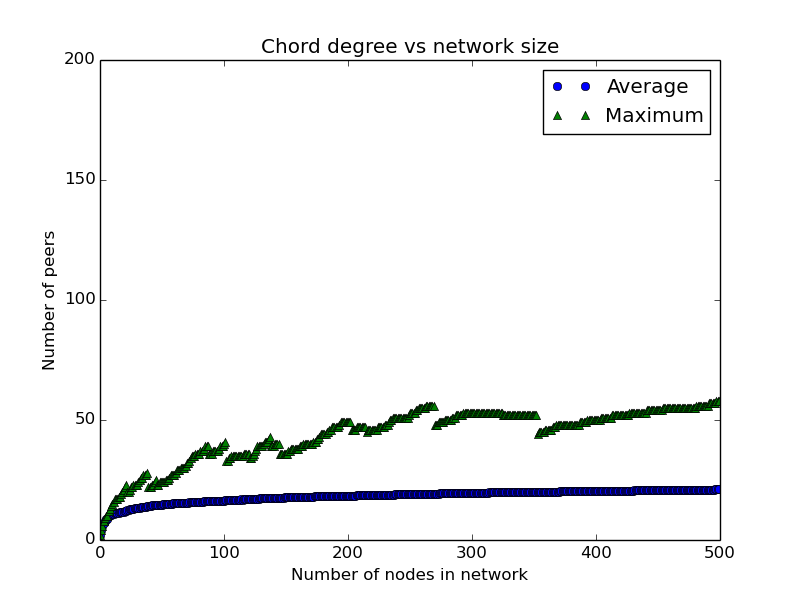
\includegraphics[width=0.7\linewidth]{figs/ChordDegree}
	\caption[Degree of nodes in Chord]{This is the average and maximum degree of nodes in the Chord network. This Chord network utilized a 120 bit hash and thus degree is bound at 122 (full fingers, predecessor and successor) when the network reaches $2^{120}$ nodes.}
	\label{fig:ChordDegree}
\end{figure}

\end{frame}

\begin{frame}{Chord Distance}
\begin{figure}
	\centering
	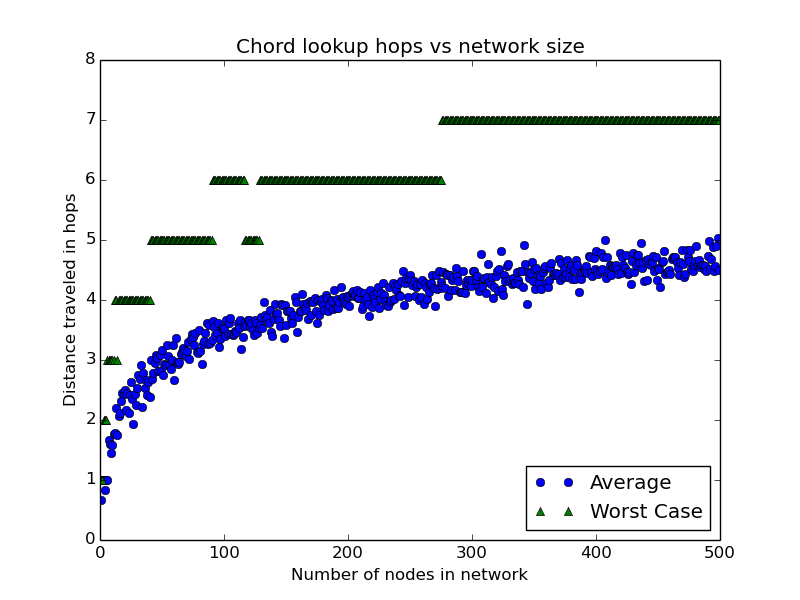
\includegraphics[width=0.7\linewidth]{figs/ChordDistance}
	\caption[Chord hops]{This is the number hops required for a greedy routed lookup in Chord. The average lookup between two nodes follows the expected logarithmic curve.}
	\label{fig:ChordDistance}
\end{figure}
\end{frame}


\begin{frame}{Kademlia Degree}
\begin{figure}
	\centering
	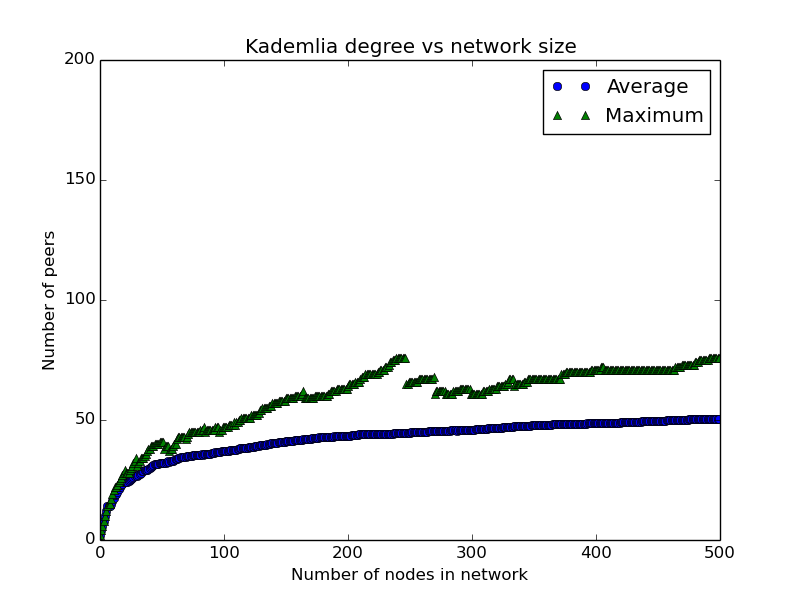
\includegraphics[width=0.7\linewidth]{figs/KademliaDegree}
	\caption[Degree of nodes in Kademlia]{This is the average and maximum degree of nodes in the Kademlia network as new nodes are added.  Both the maximum degree and average degree are $O(\log n)$.}
	\label{fig:KademliaDegree}
\end{figure}
\end{frame}

\begin{frame}{Kademlia Distance}
\begin{figure}
	\centering
	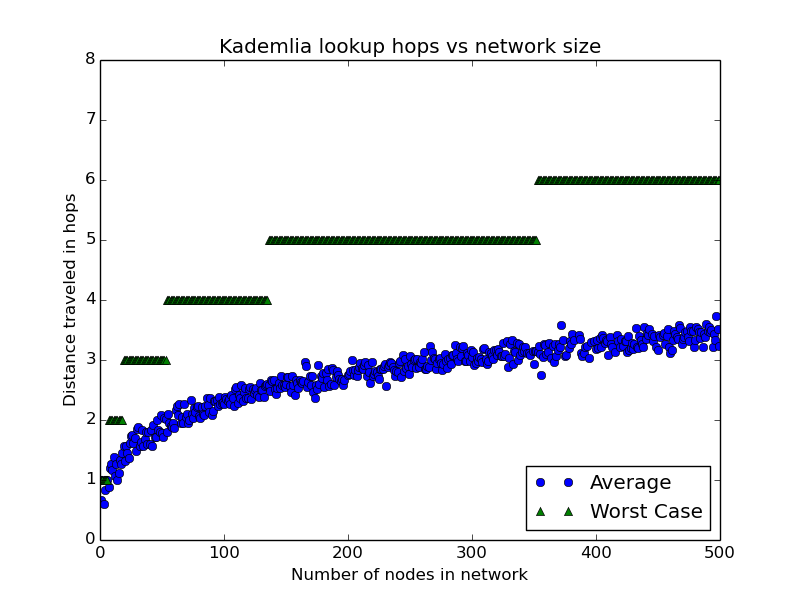
\includegraphics[width=0.7\linewidth]{figs/KademliaDistance}
	\caption[Kademlia hops]{Much like Chord, the average degree follows a distinct logarithmic curve, reaching an average distance of approximately three hops when there are 500 nodes in the network.}
	\label{fig:KademliaDistance}
\end{figure}
\end{frame}


\begin{frame}{Euclidean Degree}

\begin{figure}
	\centering
	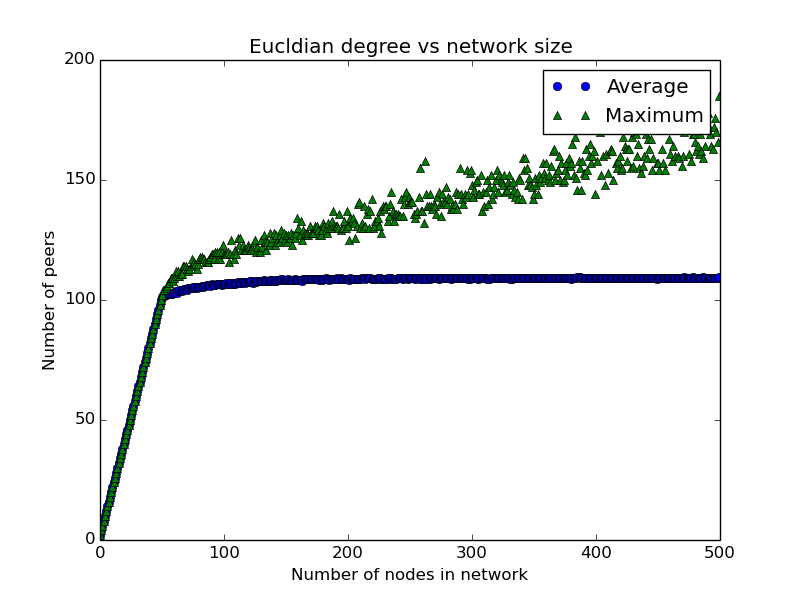
\includegraphics[width=0.7\linewidth]{figs/EucldianDegree}
	\caption[Growth of UrDHT degree]{Because the long peers increase linearly to the maximum value (49), degree initially rises quickly and then grows  more slowly as the number of long peers ceases to grow and the size short peers increases with network size. }
	\label{fig:EucldianDegree}
\end{figure}
\end{frame}

\begin{frame}{Euclidean Distance}
	\begin{figure}
		\centering
		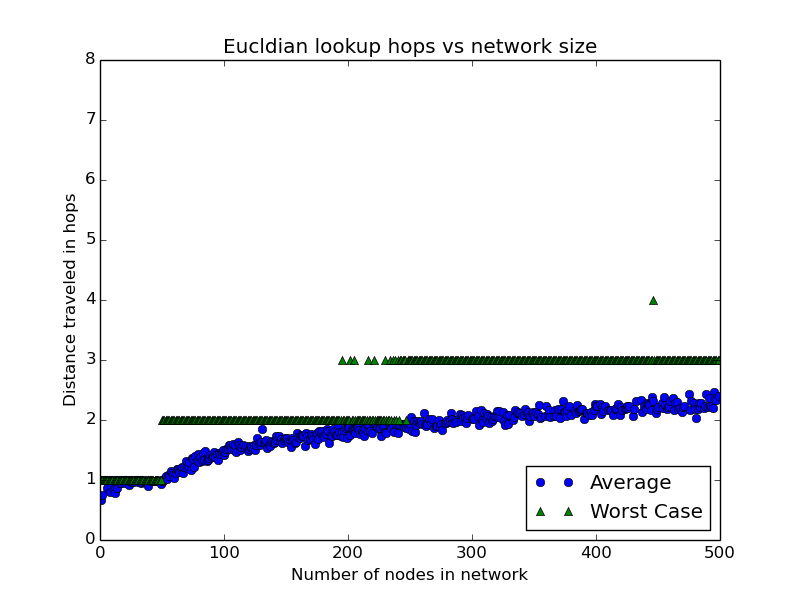
\includegraphics[width=0.7\linewidth]{figs/EucldianDistance}
		\caption[Hops in Euclidean UrDHT]{The inter-node distance stays constant at 1 until long peers are filled, then rises at the rate of a randomly connected network due to the distribution of long peers selected}
		\label{fig:EucldianDistance}
	\end{figure}
\end{frame}
	

\begin{frame}{Hyperbolic Degree}
	
	\begin{figure}
		\centering
		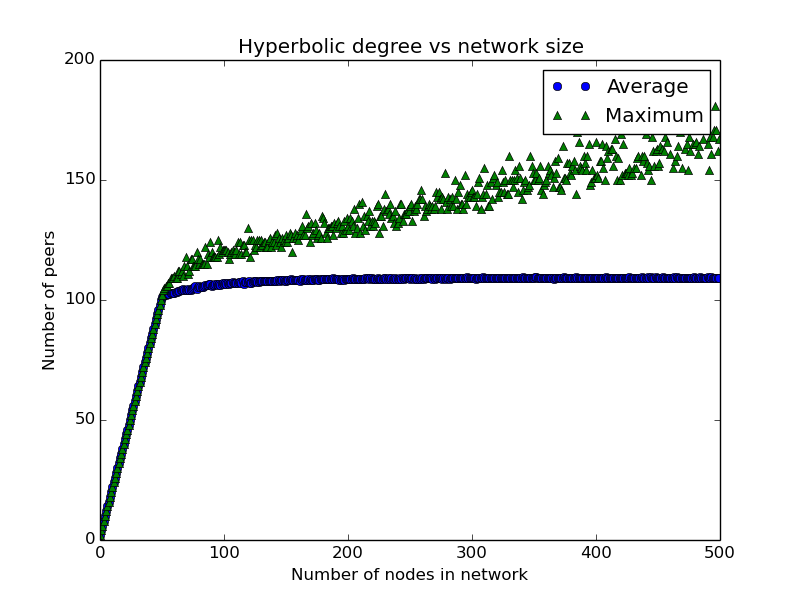
\includegraphics[width=0.7\linewidth]{figs/HyperbolicDegree}
		\caption[Growth of UrDHT degree in a hyperbolic space]{The Hyperbolic network uses the same long and short peer strategies to the Euclidean network, and thus shows similar results.}
		\label{fig:HyperbolicDegree}
	\end{figure}
\end{frame}
	

\begin{frame}{Hyperbolic Distance}
	\begin{figure}
		\centering
		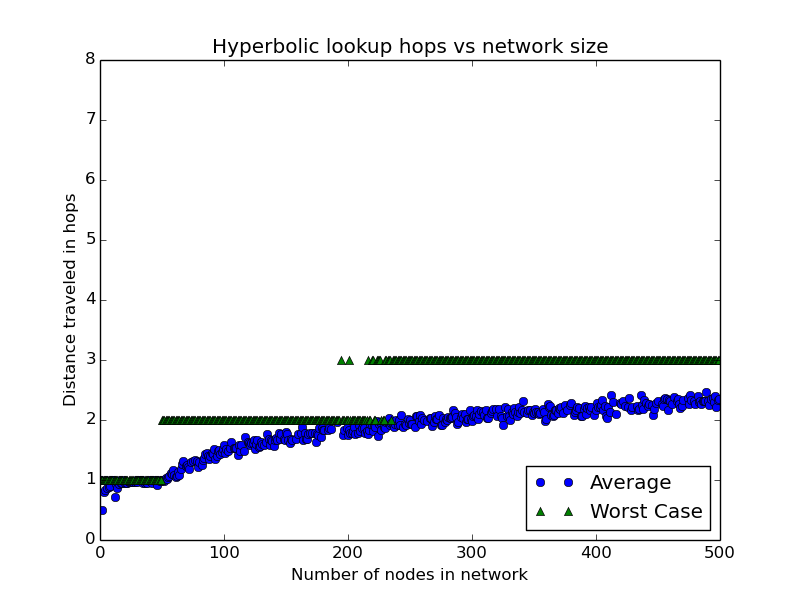
\includegraphics[width=0.7\linewidth]{figs/HyperbolicDistance}
		\caption[Hops in Hyperbolic UrDHT]{Like the Euclidean Geometry, our Poincar\`{e} disc based topology has much shorter maximum and average distances.
		}
		\label{fig:HyperbolicDistance}
	\end{figure}
\end{frame}
	



\subsection{Conclusion}

\begin{frame}{Conclusion}
\begin{itemize}
	\item UrDHT abstracts DHTs.
	\item UrDHT can emulate the topology and performance of various DHTs.
	\item We can use UrDHT to create a multidimensional DHT.
	\item The maintenance algorithm can nodes moving in the overlay.

\end{itemize}
\end{frame}

\section{Autonomous Load-Balancing}

\subsection{Introduction}
\begin{frame}{Introduction}
	\begin{itemize}
		
		\item In this project, we set out to confirm the results of ChordReduce
		\item Objectives:
		\begin{itemize}
			\item Confirm that high levels of churn can help a DHT based computing environment.
			\item Develop better strategies than randomness
		\end{itemize}
	\end{itemize}
\end{frame}


\begin{frame}{Strategies}
	\begin{itemize}
		\item Churn
		\item Random Injection
		\item Neighbor Injection
		\item Invitation
	\end{itemize}
\end{frame}




\subsection{Distribution of Keys in A DHT}


\begin{frame}{Distribution in Networks of Different Sizes}
\begin{table}
	\centering
	\caption{The median distribution of tasks (or files) among nodes.  We can see the standard deviation is fairly close to the expected mean workload ($\frac{tasks}{nodes}$). Each row is the average of 100 trials.  Experiments show there is practically little deviation in the median load of the network.}
	\begin{tabular}{r r r r}
		Nodes & Tasks & Median Workload & $\sigma$ \\ \hline
		1000 & 100000 & 69.410   &  137.27  \\
		1000 & 500000 & 346.570  &  499.169 \\
		1000 & 1000000 & 692.300  &  996.982 \\
		
		5000 & 100000  & 13.810 & 20.477 \\ 
		5000 & 500000  & 69.280 & 100.344 \\ 
		5000 & 1000000 &138.360 & 200.564 \\ 
		
		10000 & 100000 & 7.000   &  10.492 \\
		10000 & 500000 & 34.550  &   50.366 \\
		10000 & 1000000& 69.180  &  100.319 \\
	\end{tabular}
	\label{tab:medianLoads}
\end{table}

\end{frame}

\note[itemize]{
\item This means 50\% of the network has significantly less tasks than the average.  Probably more.

}


\begin{frame}{Distribution of Work in A DHT}
\begin{figure}
	\centering
	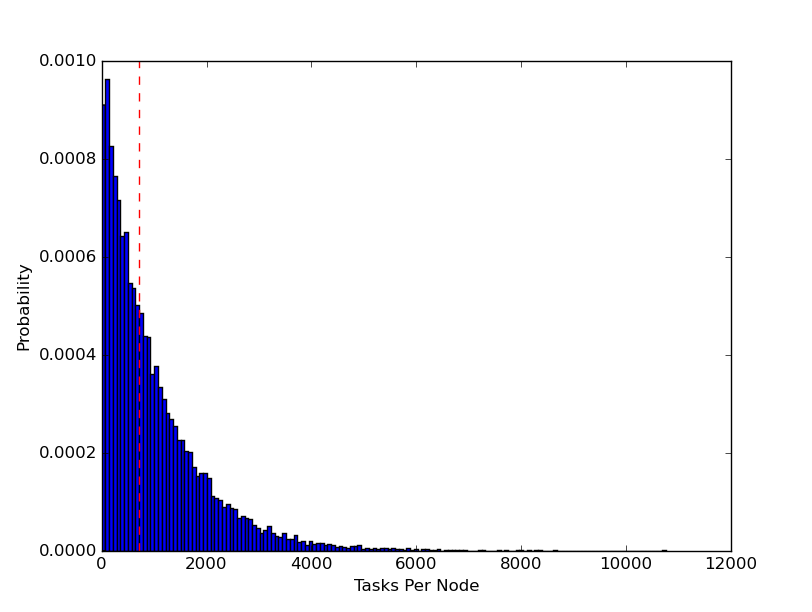
\includegraphics[width=0.7\linewidth]{figs/workloadDistribution}
	\caption[Workload Distribution in a DHT]{The probability distribution of workload in a DHT with 1000 nodes and 1,000,000 tasks or files.  The vertical dashed line designates the median.}
	\label{fig:workloadDistribution}
\end{figure}
\end{frame}

\note[itemize]{
\item Keys were generated by feeding random numbers into the SHA1 hash function, a favorite for many distributed hash tables.
\item Nodes with small amounts of work (the first two buckets)  will finish first.  
\item If each node consumes a task a tick, then that means the nodes the furthest right will dictate the runtime.
}

\begin{frame}{Distribution of Work in Chord}
\begin{figure}
	\centering
	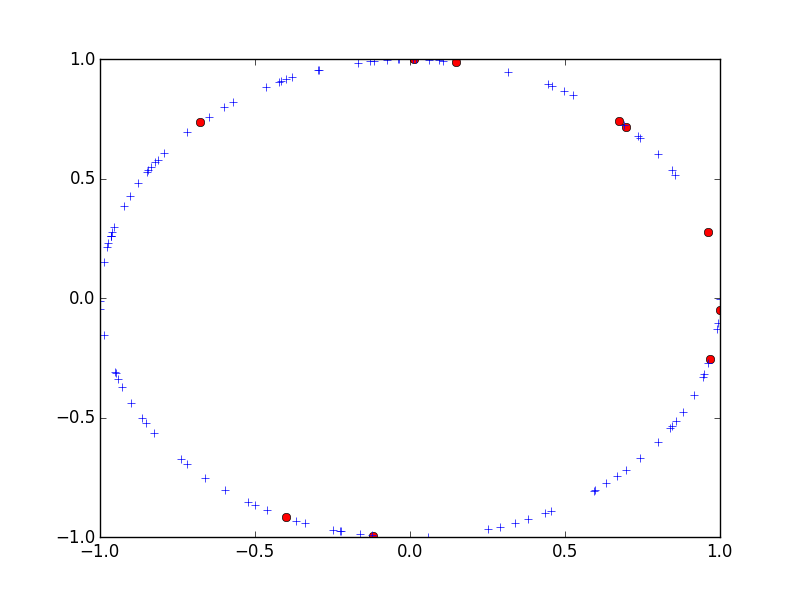
\includegraphics[width=0.7\linewidth]{figs/exampleChordDistribution}
	\caption[Distribution of Nodes and Tasks in a Chiord DHT]{A visual example of data and nodes in a Chord DHT with 10 nodes (represented by red circles) and 100 tasks (blue pluses).}
	\label{fig:exampleChordDistribution}
\end{figure}
\end{frame}

\note[itemize]{
	\item Nodes are responsible for all the tasks that fall along the perimeter between themselves and their predecessor, which is the closest node counterclockwise.
	
	\item Each node and task is given a 160-bit identifier \texttt{id} that is mapped to location $ (x,y) $ on the perimeter of the unit circle via the equations $ x = \sin\left( \frac{ 2 \pi \cdot id}{2^{160}} \right)$ and $ y = \cos\left( \frac{ 2 \pi \cdot id}{2^{160}} \right)$. 
	\item Note that some of the nodes cluster right next to each other, while other nodes have a relatively long distance between each other along the perimeter.  
	\item The most blatant example of this is the node located at approximately $(-0.67, 0.75)$, which would be responsible for all the tasks between that and the next node located counterclockwise.
	\item That node and the node located at about $(-0.1, -1)$ are responsible for approximately half the tasks in the network.
}


\subsection{Experimental Setup}
\begin{frame}{Terms and Assumptions}
	\begin{itemize}
		
		\item Time is measured in ticks.
		\item A tick is enough time to perform aggressive, reactive maintenance\footnote{This has been implemented and tested.}
		\item Jobs are measured in tasks; each task can correspond to a file or a piece of a file
		
	\end{itemize}
\end{frame}




\begin{frame}{Variables}
	\begin{itemize}
		
		\item Strategy
		\item Homogeneity 
		\item Work Measurement
		\item Number of Nodes
		\item Number of Tasks
		\item Churn Rate 
		\item Max Sybils or Node Strength
		\item Sybil Threshold 
		\item Number of Successors
	\end{itemize}
\end{frame}


\begin{frame}{Output}
	\begin{itemize}
		
		\item Ideal Runtime
		\item Runtime
		\item Runtime Factor
		\item Task Distribution
	\end{itemize}
\end{frame}

\note{
We used these to calculate a ``runtime factor,'' the ratio of the experimental runtime compared to the ideal runtime.
For example, in the network from our previous example took 852 ticks to finish, its factor is 8.52.
We prefer to use this runtime factor for comparisons since it allows us to compare networks of different compositions, task assignments, and other variables.

}

\subsection{Churn}
\begin{frame}{Strategy}
	\begin{itemize}
		
		\item The network load-balances using churn
		\item \texttt{churnRate} chance per tick for each node to leave network
		\item Pool of potentially joining joins at the same rate
	\end{itemize}
\end{frame}

\note[itemize]{
	\item Leaving nodes enter pool, joing nodes leave pool
	\item Check is done before work is done
}


\begin{frame}{Runtime}
	\begin{table}[h]
		\tiny
		\centering
		\caption[Churn Runtimes in a homogenious network]{Runtime factor of networks of varying sizes and number of tasks, each using the Churn strategy to load-balance.  Each result is the average of 100 trials. The networks are homogeneous and each node consumes one task per tick.  A runtime of 1 is the ideal and target.}
		\begin{tabular}{|p{1cm} || p{1cm} | p{1cm} | p{1cm} | p{1cm} | p{1cm} |}
			\hline
			Churn Rate & $ 10^{3}$ nodes, $ 10^{5}$ tasks & $ 10^{3}$ nodes, $ 10^{6}$ tasks & $ 100$ nodes, $ 10^{4}$ tasks & $ 100$ nodes, $ 10^{5}$ tasks &$ 100$ nodes, $ 10^{6}$ tasks \\ \hline
			0      & 7.476   &  7.467 &  5.043& 5.022 &5.016 \\\hline
			0.0001 & 7.122   &  5.732 &  4.934& 4.362&3.077 \\\hline
			0.001  & 6.047   &  3.674 &  4.391& 3.019  &1.863\\\hline
			0.01  &  3.721   &  2.104 &  3.076& 1.873 &1.309\\\hline
			
		\end{tabular}
		\label{tab:ChurnRuntimesHomogenious}
	\end{table}
\end{frame}

\note[itemize]{
	\item The magnitude of churn's effect varies based on the size of the network and the number of tasks. 
	\item In networks where there are fewer nodes, we see the base runtime factor is smaller.
	\item The more tasks there are, the greater the gains of churn.
	\item A network 100 nodes and 1 million tasks, on average, has a runtime factor only 30\% higher than ideal when churn is 0.01 per tick.
	\item The runtime for heterogeneous versus homogeneous networks had no significant differences.  This won't always be the case.}


\begin{frame}{Churn vs Runtime factor}
	\begin{figure}[h]
		\centering
		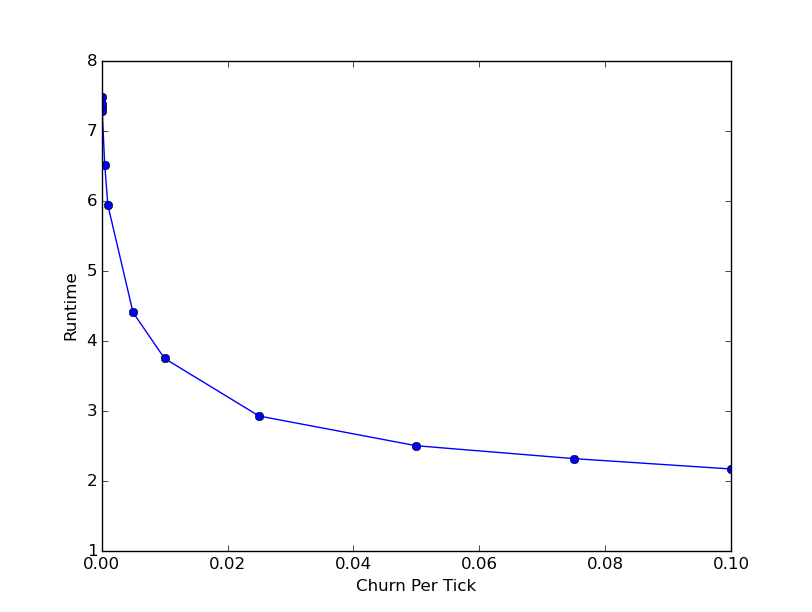
\includegraphics[width=0.7\linewidth]{figs/churnVsTime}
		\caption[Churn vs Runtime factor]{This graph shows the effect churn has on runtime in a distributed computation.
			Runtime is measured as how many times slower the computation runs than an ideal computation, where each node receives an equal number of tasks.
			The lower the runtime factor, the closer it is to an ideal of 1.
			Neither the homogeneity of the network nor work measurement had a significant effect on the runtime.}
		\label{fig:churnVsTime}
	\end{figure}
\end{frame}


%\begin{frame}{Churn vs Average Work Per Tick}
%\begin{figure}
%	\centering
%	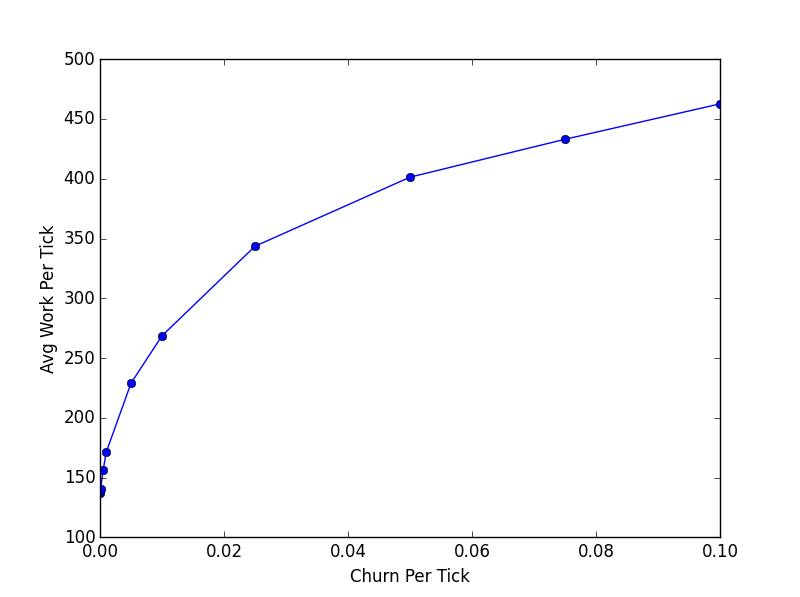
\includegraphics[width=0.7\linewidth]{figs/churnVsWork}
%	\caption[Churn vs average work per tick]{With more and more churn in the network, new nodes have a higher chance of joining the network and acquiring work from overloaded nodes.  This results in more average work being done each tick, as there are less nodes simply idling.}
%	\label{fig:churnVsWork}
%\end{figure}
%
%\end{frame}

\begin{frame}{Base Work Distribution}
\begin{figure}
	\centering
	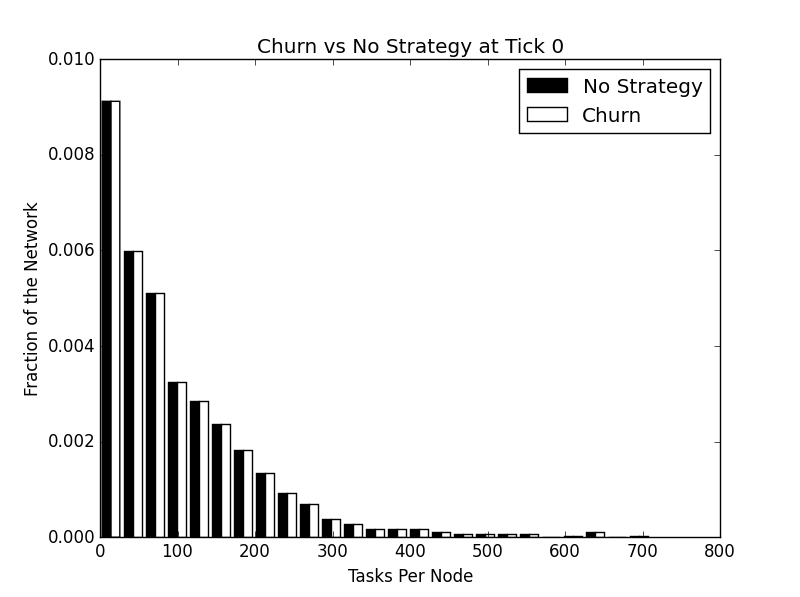
\includegraphics[width=0.7\linewidth]{figs/ChurnStableHist0}
	\caption[Workload for churn at tick 0]{The initial distribution of the workload in both networks.  As both networks start with same initial configuration, the distribution is currently identical.  This greatly resembles the distribution we saw in Figure \ref{fig:workloadDistribution}.}
	
	\label{fig:churnStableHist0}
\end{figure}
\end{frame}

\note{This will be the same for every strategy.}



\begin{frame}{Churn Distribution after 35 Ticks}
\begin{figure}
	\centering
	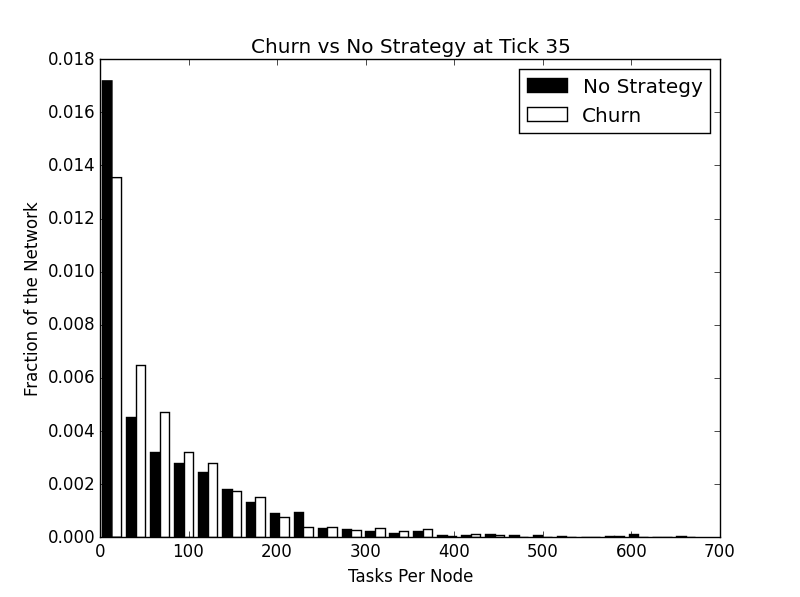
\includegraphics[width=0.7\linewidth]{figs/ChurnStableHist35}
	\caption[Workload for churn at tick 35]{After 35 ticks, the effects of churn on the workload distribution become more pronounced.  More nodes have consumed all their tasks and are simply idling, but significantly less in the network using churn.}
	\label{fig:churnStableHist35}
\end{figure}
\end{frame}

\begin{frame}{Remarks}
\begin{itemize}
	\item Diminishing returns
	\item Maintenance costs can get excessive
	\item We don't actually have to kill nodes, most of the speedup is from joining.
\end{itemize}
\end{frame}


\subsection{Random Injection}
\begin{frame}{Strategy}
	\begin{itemize}
		
		\item Nodes with loads $ \leq $ \texttt{sybilThreshold} create Sybils
		\item This check occurs every 5 ticks before work is performed
		\item These Sybils are randomly placed
		\item Act as a virtual node so the same node essentially exists in multiple locations
		\item Sybils are removed if the node that created it has no work
		
	\end{itemize}
\end{frame}

\note[itemize]{
	\item Leaving nodes enter pool, joing nodes leave pool
	\item Sybil removal is instantaneous if no qork was acquired.  We can get a similar result with no disruption if a node asks if it would be stealing any work.
}

\begin{frame}{Effects of Network Size}
	\begin{itemize}
		\item A homogeneous, 1000 node/100,000 task network, never have an average runtime factor greater than 1.7
		\item Minimum was 1.36.
		\item In the same network with 1,000,000 tasks, these runtimes were 1.25 and 1.12 respectively.
		\item On average, the 1,000,000 task network had a runtime factor 0.82 less than the 100,000 task network.
	\end{itemize}
\end{frame}

\note[itemize]{
\item  	Heterogeneous networks also saw signifcantly better performance , but the gains were not as great as in homogeneous networks.
\item However, the larger ratio networks handled heterogeneity much better, with the worst average heterogeneous run time being 1.955 in networks with
1000 tasks per node, compared to 4.052 on the smaller ratio networks with 100 tasks per node.
\item Most trials did not have a runtime factor greater than 3.
\item Random injection handled heterogeneity the best
}


\begin{frame}{Random Injection vs No Strategy After 35 ticks}
\begin{figure}
	\centering
	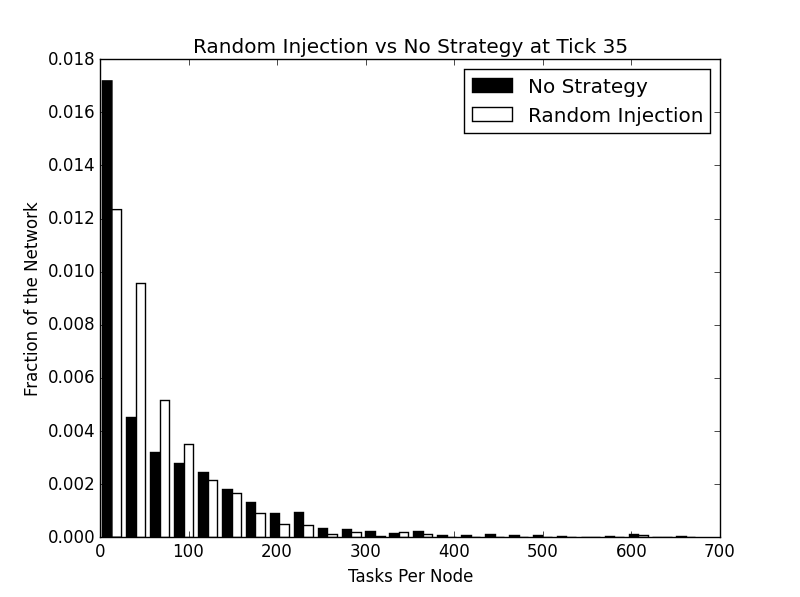
\includegraphics[width=0.7\linewidth]{figs/randomStableHist35}
	\caption[Random injection vs no strategy after 35 ticks.]{The networks after 35 ticks.  The network using random injection has significantly less underutilized nodes and substantially more notes with some or lots of work.}
	\label{fig:randomStableHist35}
\end{figure}
\end{frame}

\note[itemize]{
	\item We see even better improvement here.
}


\begin{frame}{Random Injection in a Heterogeneous Network}
\begin{figure}
	\centering
	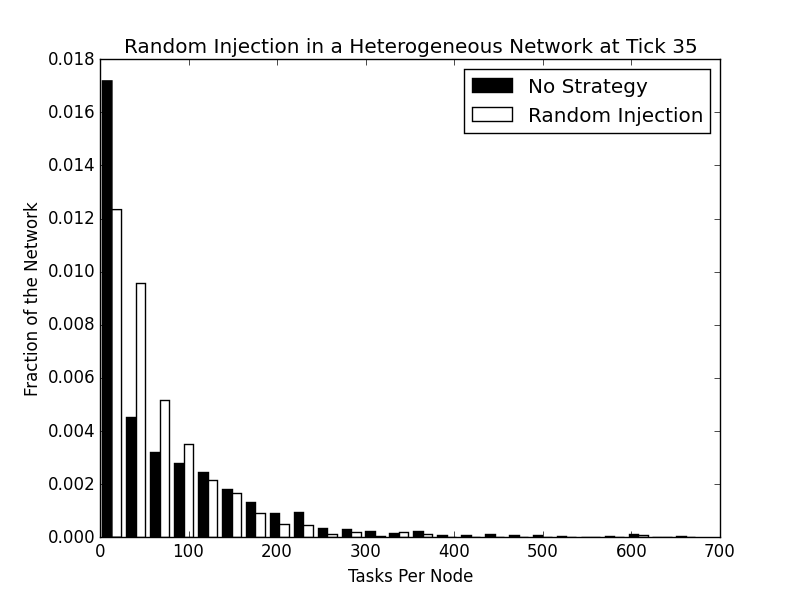
\includegraphics[width=0.7\linewidth]{figs/randomStableHistHetero35}
	\caption[Random injection in a Heterogenous Network]{The workload distribution of heterogenous networks after 35 ticks.  }
	\label{fig:randomStableHistHetero35}
\end{figure}
\end{frame}
\note[itemize]{
	\item We can see the network using the random injection strategy is experiencing a better distribution of work.
	\item This did not translate to better runtime factor, as we'll in in other experiments.
}



\begin{frame}{Random Injection VS Churn}
\begin{figure}
	\centering
	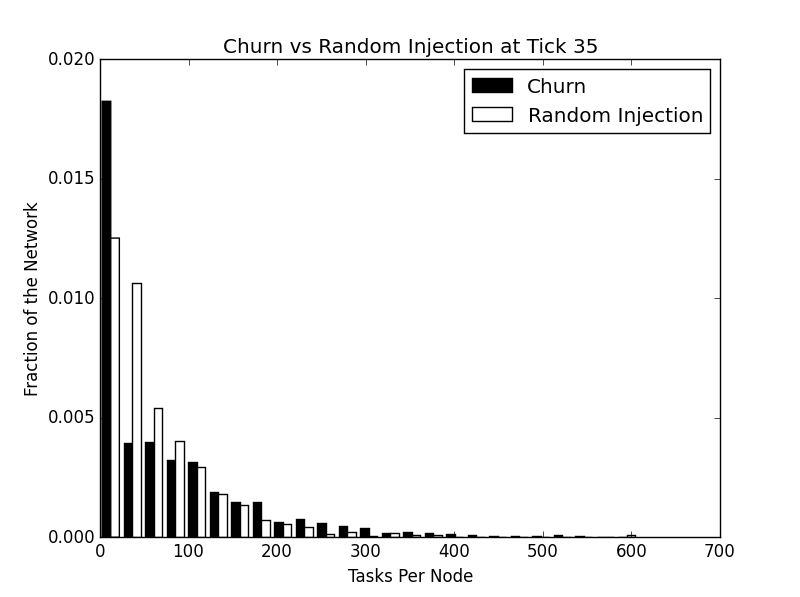
\includegraphics[width=0.7\linewidth]{figs/churnInjectionHist35}
	\caption[Churn vs Random Injection after 35 ticks.]{The networks after 35 ticks.  The network using random injection load-balances significantly better than the network using Churn.}
	\label{fig:churnInjectionHist35}
\end{figure}

\end{frame}




\begin{frame}{Impacts of Variables}
	\begin{itemize}
		\item \texttt{sybilThreshold} would lower the runtime factor.  
		\item Churn had no significant effect.
		\item \texttt{maxSybils} (node strength) had no effect in homogeneous networks.
	\end{itemize}
\end{frame}

\note[itemize]{
\item \texttt{sybilThreshold} did nothing in heterogeneous networks. The improvement was tied to the ratio of tasks to nodes.
\item  Heterogeneous networks were hurt by \texttt{maxSybils} being larger.  The wider the disparity in strength, the more the network was hurt.
}

\begin{frame}{Remarks}
	\begin{itemize}
		\item Best runtime factor of our experiments.
		\item Could still incur high maintenance costs, especially with nodes being deleted as soon as they are made.
	\end{itemize}
\end{frame}



\note[itemize]{
\item Gets extremely close to ideal.
\item Query first
}



\subsection{Neighbor Injection}
\begin{frame}{Strategy}
	\begin{itemize}
		\item Rather than creating Sybils randomly, nodes create one in their successors
		\item Finding node id uses mashes
		\item Estimates which successor has most work.
		\item Tested estimation against smart method.
	\end{itemize}
\end{frame}

\note[itemize]{
	\item Smart actually queuries
	\item Estimation can cause a node to keep checking same space each tick.  Trivial to solve.
	\item Otherwise same as random injection
}

\begin{frame}{Base Runtime}
\begin{itemize}
	\item The base runtime in a 1000 node/100,000 task homogeneous network was 5.033
	\item 2.4 lower than no strategy
	\item Base runtime in a heterogeneous runtime was worse
	\item \texttt{numSuccessors} improves the runtime factor (0.3 for base network)
	\item Other variables had no significant effect.
\end{itemize}
\end{frame}

\note{This is because the network is finishing off the tasks with small amounts of work quicker.
	However, nodes are not able to acquire work outside their immediate vicinity and must idle.
	In addition, nodes always inject Sybils into the largest gap between their successors that they see, but if they acquire no work.
	That means in the simulation, it is possible for nodes to get into a loop of constantly checking the largest gap and miss other neighbors that do have work to acquire.
}



%\begin{frame}{Neighbor Injection after 5 Ticks}
%\begin{figure}
%	\centering
%	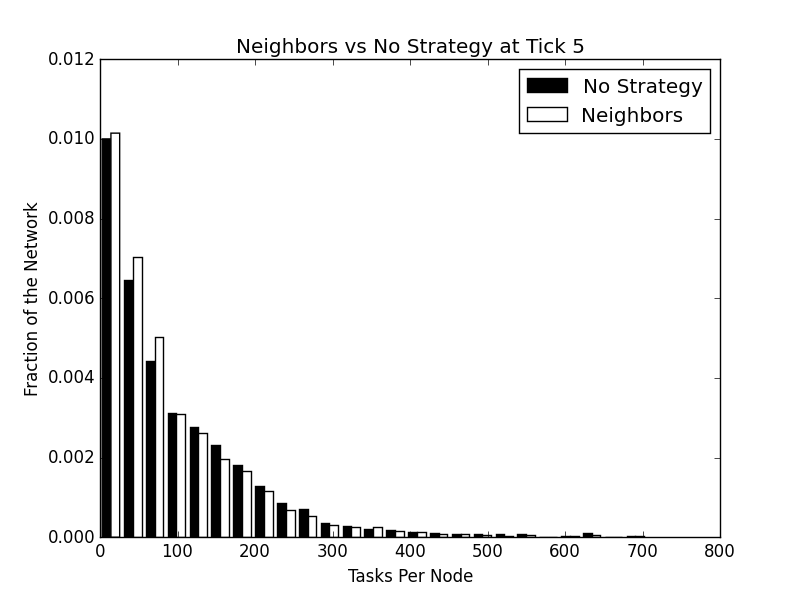
\includegraphics[width=0.7\linewidth]{figs/neighborsStableHist5}
%	\caption[Neighbor injection vs no strategy after 5 ticks.]{While the network no strategy appears to have less nodes idling, the active nodes in the network using neighbors are being better utilized.}
%	\label{fig:neighborsStableHist5}
%\end{figure}
%
%
%\end{frame}
%
%
%\note{At the first glance, neighbor injection does not seem to be doing worse than no strategy; there are more nodes with less work than no strategy.
%	However, if we look at the whole histogram, we see there are less nodes that have a huge amount of work and noticeably more nodes with a small number of tasks.
%	In fact, at tick 35, we see that the network with no strategy has a node with approximately 650 tasks, while the most the network using the neighbors strategy has is 450 tasks.}

\begin{frame}{Neighbor Injection after 35 Ticks}
\begin{figure}
	\centering
	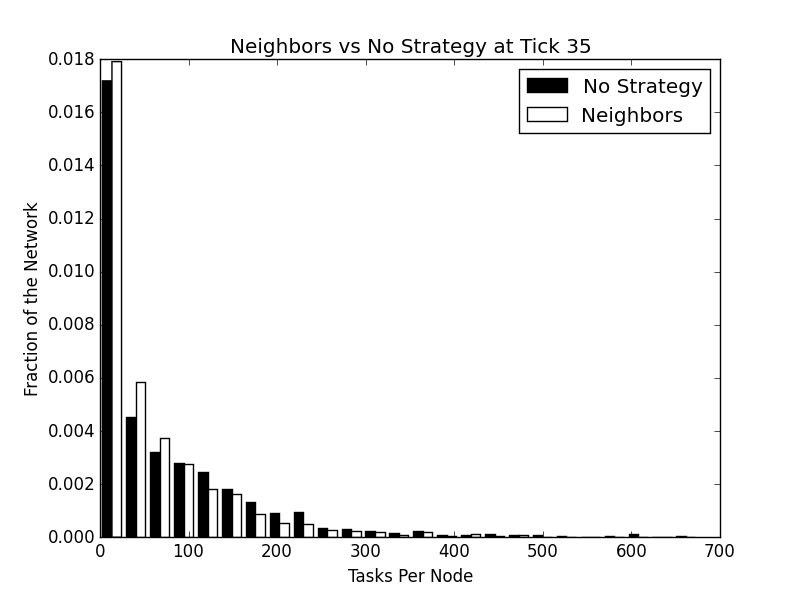
\includegraphics[width=0.7\linewidth]{figs/neighborsStableHist35}
	\caption[Neighbor injection  vs no strategy after 35 ticks.]{Despite have more idling nodes, we see that the nodes using the neighbor injection strategy have acquired smaller workloads and have effectively shifted part of the histogram left.}
	\label{fig:neighborsStableHist35}
\end{figure}

\end{frame}



\begin{frame}{Smart Neighbor Injection after 35 Ticks}
\begin{figure}
	\centering
	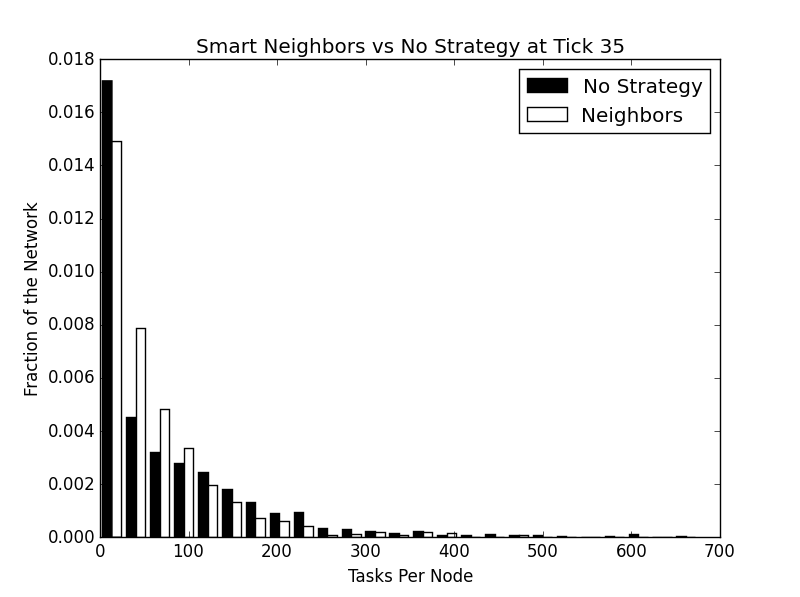
\includegraphics[width=0.7\linewidth]{figs/neighborsStableSmartHist35}
	\caption[Smart Neighbor injection  vs no strategy after 35 ticks.]{After 35 ticks, we see the network using the smart neighbor injection strategy has significantly less nodes with little or no work, more nodes with smaller amounts of work, and less nodes with large amounts of tasks.}
	\label{fig:neighborsStableSmartHist35}
\end{figure}
\end{frame}



\begin{frame}{Remarks}
	\begin{itemize}
		\item Smart method improved runtime factor by 1.2 on average.
		\item Smart would require querying, ``dumb'' estimation still would provide improvement.
		\item Less churn of joining nodes.
	\end{itemize}
\end{frame}

\subsection{Invitation}
\begin{frame}{Strategy}
	\begin{itemize}
		\item Nodes with too much work ask for help.
		\item Predecessor with smallest workload and below \texttt{sybilThreshold} creates a Sybil.
		\item Reactive vs Proactive.
	\end{itemize}
\end{frame}

\note[itemize]{
	\item Only checks to create more work when a node is actually over loaded
	\item This means less traffic
	\item Random and neighbors try to acquire work proactively
	\item They spam new sybils in the hopes of finding a place to grab work from
	\item Invitation is reactive, overloaded nodes react and ask for sybils
	\item less churn
}




\begin{frame}{Invitation at 35 Ticks}
\begin{figure}
	\centering
	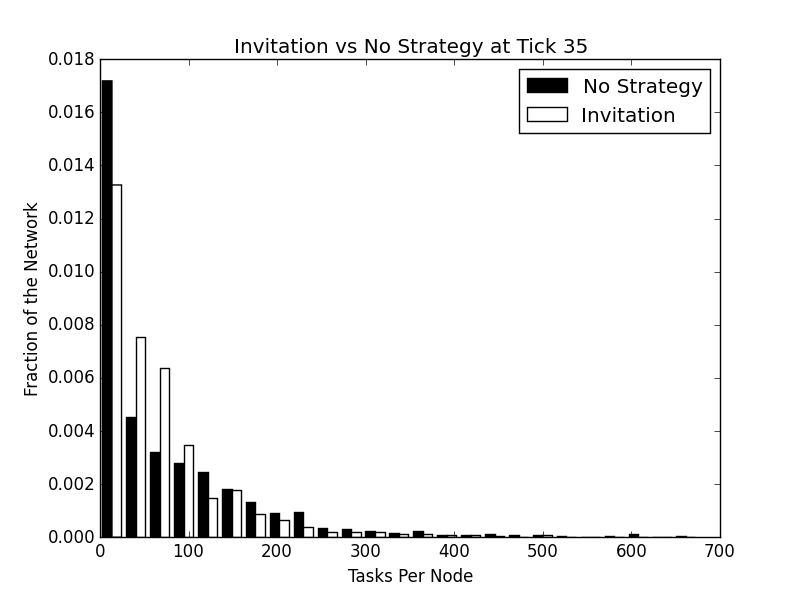
\includegraphics[width=0.7\linewidth]{figs/inviteStableHist35}
	\caption[Invitiation vs no strategy after 35 ticks]{At 35 ticks, we can see the network using the invitation strategy perform markedly better than the network using no strategy. The highest load is around 500 tasks in the network using invitation, compared to approximately 650 tasks in the network using no strategy.}
	\label{fig:inviteStableHist35}
\end{figure}
\end{frame}




\begin{frame}{Invitation vs Smart Neighbors at Tick 35}

\begin{figure}
	\centering
	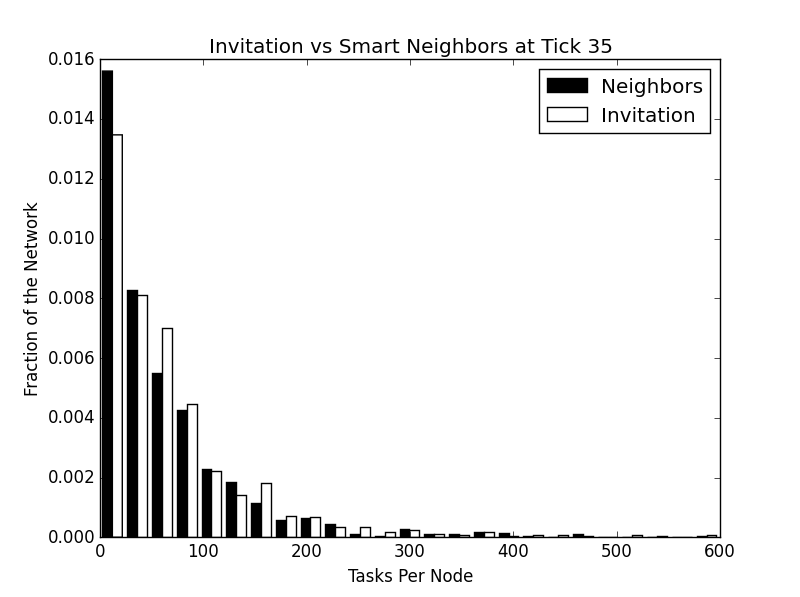
\includegraphics[width=0.7\linewidth]{figs/inviteNeighborsHist35}
	\caption[Invitation vs smart neighbor injection after 35 ticks.]{After 35 ticks, differences between the two strategies have emerged.  The network using the invitation strategy has significantly less nodes with a small work load and many more with large work loads.}
	\label{fig:inviteNeighborsHist35}
\end{figure}

\end{frame}



\begin{frame}{Remarks}
	\begin{itemize}
		\item Impact of Invitation was closely tied to the number of nodes in the network.
		\begin{itemize}
			\item 100 node/ 100,000 task network (1000 tasks per node), the base average runtime factor was 3.749.
			\item 1000 node/ 100,000 task network had a base average runtime of 5.673.
		\end{itemize}
		\item Performed poorer in heterogeneous networks, but better than base on average (6.097 vs 7.5).
		\item Better than smart neighbors and uses less bandwidth.
	\end{itemize}
\end{frame}

\subsection{Conclusion}

\begin{frame}{Summary}
	\begin{itemize}
		
		\item Reactive vs Proactive
		\item Heterogeneity was best handled by Churn or Random Injection.
		\item Random injection was best overall
		\item Load balanced did not mean faster since node strength was not taken into account.
	\end{itemize}
\end{frame}

\section{Conclusion}

\subsection{Conclusion}

\begin{frame}{Conclusion}
	\begin{itemize}
		
		\item Load Balancing
	\end{itemize}
\end{frame}



\begin{frame}{Publication List}
	\begin{itemize}
		
		\item Load Balancing
	\end{itemize}
\end{frame}

%\subsection{Publications}
%\begin{frame}{Published Work}
% 	\begin{itemize}\tiny{
%		\item Andrew Rosen, Brendan Benshoof, Robert W. Harrison, Anu G. Bourgeois ``MapReduce on a Chord Distributed Hash Table'' Poster at IPDPS 2014 PhD Forum
%		\item Andrew Rosen, Brendan Benshoof, Robert W. Harrison, Anu G. Bourgeois ``MapReduce on a Chord Distributed Hash Table'' Presentation ICA CON 2014
%		\item Brendan Benshoof, Andrew Rosen, Anu G. Bourgeois, Robert W. Harrison ``VHASH: Spatial DHT based on Voronoi Tessellation'' Short Paper ICA CON 2014 
%		\item Brendan Benshoof, Andrew Rosen, Anu G. Bourgeois, Robert W. Harrison ``VHASH: Spatial DHT based on Voronoi Tessellation'' Poster ICA CON 2014 
%		\item Brendan Benshoof, Andrew Rosen, Anu G. Bourgeois, Robert W. Harrison ``A Distributed Greedy Heuristic for Computing Voronoi Tessellations With Applications Towards Peer-to-Peer Networks'' IEEE IPDPS 2015 - Workshop on Dependable Parallel, Distributed and Network-Centric Systems}
%	\end{itemize}
%	
%\end{frame}
%
%
%\begin{frame}{In Progress}
%	\begin{itemize}\footnotesize{
%		\item Brendan Benshoof, Andrew Rosen, Anu G. Bourgeois, Robert W. Harrison ``UrDHT: A Generalized DHT''
%		\item Andrew Rosen, Brendan Benshoof, Robert W. Harrison, Anu G. Bourgeois ``The Sybil Attack on Peer-to-Peer Networks From the Attacker's Perspective''
%		\item Chaoyang Li, Andrew Rosen, Anu G. Bourgeois ``On Minimum Camera Set Problem in Camera Sensor Networks''}
%	\end{itemize}
%\end{frame}
%
%\begin{frame}{Other Publications}
%	
%	\begin{itemize}
%		\footnotesize{
%		\item  Erin-Elizabeth A. Durham, Andrew Rosen, Robert W. Harrison
%		``A Model Architecture for Big Data applications using Relational Databases''
%		2014 IEEE BigData - C4BD2014 - Workshop on Complexity for Big Data  
%		\item Chinua Umoja, J.T. Torrance, Erin-Elizabeth A. Durham, Andrew Rosen, Dr. Robert Harrison
%		``A Novel Approach to Determine Docking Locations Using Fuzzy Logic and Shape Determination''
%		2014 IEEE BigData - Poster and Short Paper 
%		\item  Erin-Elizabeth A. Durham, Andrew Rosen, Robert W. Harrison
%		``Optimization of Relational Database Usage Involving Big Data'' 
%		IEEE SSCI 2014 - CIDM 2014 - The IEEE Symposium Series on Computational Intelligence and Data Mining }
%	\end{itemize}
%\end{frame}
\end{document}
